Before we start with this problem, let's review what the \EnergyInteractionModel{} does for us. As we have said before, conservation of energy relates values of certain physical parameters at the beginning of a process to the values of those parameters at the end of the process. The parameters are typically the indicators of the energy systems that change during the process or interaction. If we have a question about -- or want to predict values for -- some parameter and this parameter happens to be an indicator of an energy system, or a coefficient in an expression for an energy system, then we can proceed to construct a particular model and see if it gets us what we want.\\

\begin{wrapfigure}{R}{.2\textwidth}
	\centering
	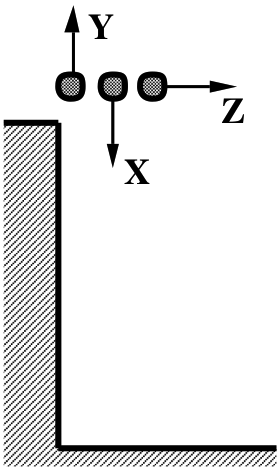
\includegraphics[width=.98\linewidth]{fnt211-rocksxyz}	
\end{wrapfigure}

\label{fnt2.1.1-1}

\noindent\textbf{The Phenomena}: Three rocks of equal mass are thrown with identical speeds from the top of the same building. (1) Rock X is thrown vertically downward, (2) Rock Y is thrown vertically upward, and (3) Rock Z is thrown horizontally.\\

\noindent\textbf{The Question}: Which rock has the greatest speed just before it hits the ground? Assume air resistance is negligible.\\

\noindent How can we determine this? We could take a guess, but it helps our argument if it is possible to apply the \EnergyInteractionModel{}. The prompts below will guide you through the process.

\begin{enumerate}[(a)]
	\item Let's start by making a prediction based on your prior experience. Don't waste a lot of time on this right now, but it's useful to give it some thought. We will definitely come back to this at the end in \hyperref[fnt211-1f]{Part~(\ref*{fnt211-1f})}. Your first, intuitive ideas might be very useful!
	\label{fnt211-1a}
	
	\item Does the question involve a parameter that you know to be an indicator of the change in an energy system? Which energy system and what is the indicator?
	\label{fnt211-1b}
	
	\item \textbf{Rock X}: Construct an \EnergyDiagram{} for Rock X, which is thrown straight down. Write out the expression for energy conservation, based on your \EnergyDiagram{}, as $\Delta E$'s; then substitute in algebraic symbols for the different energy systems. We are \emph{not} asking to go any further, but if you ``just have to,'' go ahead and try solving it for the final speed, $v_f$ (but you \emph{really} don't need to).
	\label{fnt211-1c}
	
	\item \textbf{Rock Y}: Now, without actually writing anything down, consider what would be different in your \EnergyDiagram{} for Rock Y. How about the algebraic representation -- anything different?  Go back and re-read the ``The Phenomena'' description at the beginning of the FNT, if you are not sure. Is there anything different in terms of what goes into the model? In terms of the \EnergyInteractionModel{} are there any differences?  Yes or No? Are you 100\% sure? Why?
	\label{fnt211-1d}
	
	\item \textbf{Rock Z}: Repeat for Rock Z. Any differences in the model?  Yes or No?
	\label{fnt211-1e}
	
	\item Do you believe that conservation of energy holds true for these three phenomena? Another way to ask this: Does the {\em particular energy model} you developed apply to all three cases?  If yes, what does conservation of energy tell you about the final \textbf{\em speeds} of the three rocks with 100\% confidence?
	\label{fnt211-1f}
	
	\item How do you reconcile your result in \hyperref[fnt211-1f]{Part~(\ref*{fnt211-1f})} with your initial ideas from \hyperref[fnt211-1a]{Part~(\ref*{fnt211-1a})} above?  They are not crazy, because there are indeed very obvious differences in the three situations. Why don't these differences matter to energy conservation?  Try to be as explicit here as you can be. This is what we will focus on in the FNT follow-up in DL.
	\label{fnt211-1g}
\end{enumerate}